\section*{Generic sort}

Today we will explore the difference between \lstinline'void*' in C0
and \lstinline'void*' in C, and exploit that difference to write a
generic sort in C.
\begin{center}\vspace{-1ex}
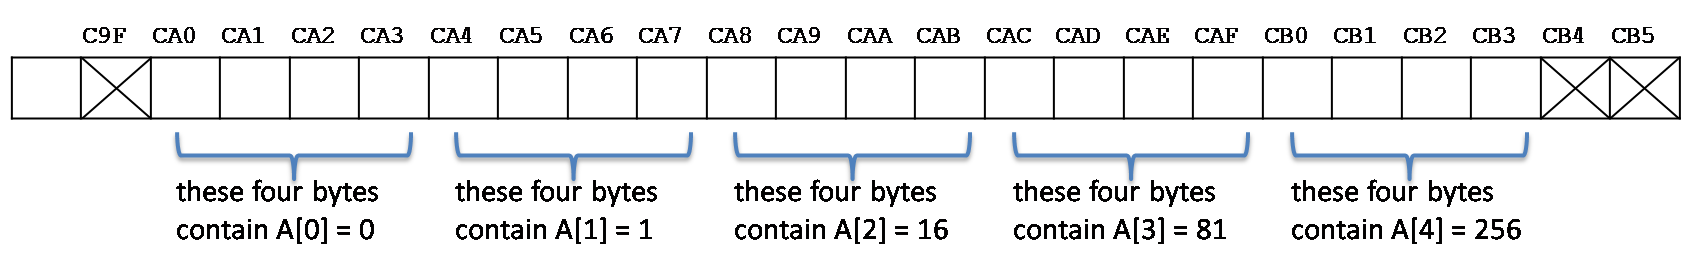
\includegraphics[width=\textwidth]{\img/allocation.png}
\end{center}\vspace{-1ex}
The image above shows a 16 byte allocation where each byte contains an
8-bit value. The actual size of a byte in C is implementation-defined
and so can be 8 bits \emph{or more}.  You can pretty much count on a
byte being 8 bits on current computers.

If we have a pointer \lstinline'A' whose value is \lstinline'0xB58',
then the way we interpret that pointer \emph{depends on the type of
  the pointer}.  As a \lstinline'char*', the pointer \lstinline'A'
points to the value \lstinline'0x48' or \lstinline"'H'", the first
character in the \lstinline'NUL'-terminated string %
\lstinline'"Hello, everyone"'.  %
As an \lstinline'int32_t*', the pointer \lstinline'A'
points to a signed integer, the first element in an array of four
integers. (According to the implementation-defined behavior we usually
expect, this array contains the four integers 1819043144, 1696607343,
2037540214, and 6647407.) If \lstinline'A' is a \lstinline'void*',
then we know \emph{nothing} about how to interpret, read from, or
write to this block of memory.

In this lab, we will write a function that sorts arrays without
knowing anything about how to interpret, read from, or write to the
memory addresses in that array. The client will tell us the how many
elements there are (\lstinline'count') and the size of each element
(\lstinline'elt_size'). The client will also tell us how to interpret
(with a comparison function) and manipulate (with a swap function)
elements of the array.

\enlargethispage{5ex}
\begin{lstlisting}[numbers=none, belowskip=0pt]
typedef void swap_fn(void *x, void *y)
  /*@requires x != NULL && y != NULL; @*/ ;

// Compares the values at memory locations x and y
typedef int compare_fn(void *x, void *y)
  /*@requires x != NULL && y != NULL; @*/
  /*@ensures -1 <= \result && \result <= 1; @*/ ;

void gsort(void *A, size_t count, size_t elt_size,
           swap_fn *swp, compare_fn *cmp)
  /*@requires A != NULL && swp != NULL && cmp != NULL; @*/
  /* requires that A is an allocation of at least count * elt_size */ ;
\end{lstlisting}

The interface above is provided in \lstinline'lib/gsort.h'.  Your
implementation in \lstinline'gsort.c' is one of the very small number
of cases in C where it is acceptable to cast a \lstinline'void*' to
another pointer type without being absolutely certain what type the
\lstinline'void*' originally was. (Remember that it was \emph{never}
acceptable to do this in C1.)

If a client asks us to sort the 5 two-byte values starting at the
\lstinline'void' pointer \lstinline'0xB58', then we know that the five
elements in the array have the addresses \lstinline'0xB58',
\lstinline'0xB5A', \lstinline'0xB5C', \lstinline'0xB5E', and
\lstinline'0xB60'. We can calculate the address of the array element
that the client thinks of as \lstinline'A[3]' by casting \lstinline'A'
to a \lstinline'char*' and then writing either \lstinline'(A + 6)' or
\lstinline'&A[6]'. This makes sense because a \lstinline'char' is
always one byte and because 6 is the array offset (3) times the size
of an array element in bytes (2).

\onePT

All we need to do to sort is calculate the addresses where array
elements begin and pass these addresses to the client functions. The
client's functions know how to compare and swap values given the
addresses of those values.  Because you are writing the sorting
algorithm without knowing what values are being stored, you shouldn't
ever access the memory in the array directly.

\begin{part}\TAGS{c-array, c-memory, function-pointer, genericity, sorting, void-star}
  Write a generic sort in \lstinline'gsort.c' according to the
  strategy described above. Make sure your \lstinline'gsort.c'
  includes \lstinline'"lib/gsort.h"'. A C0 version of selection sort
  is given to you below and in \lstinline'sort.c0'. Don't worry about
  translating the contracts.  You can test your code by running:
\begin{lstlisting}[language={[coin]C}]
% make
% ./a.out
\end{lstlisting}

\twoPT

\begin{solution}
\begin{lstlisting}[language=C]
#include <stdlib.h>
#include <stdbool.h>
#include "lib/gsort.h"
#include "lib/contracts.h"

void gsort(void *A, size_t count, size_t elt_size, swap_fn *s, compare_fn *c) {
  REQUIRES(A != NULL && s != NULL && c != NULL);

  swap_fn *swap = s;
  compare_fn *compare = c;
  char* B = A;

  for (size_t i = 0; i < count * elt_size; i += elt_size) {
    char* min = B+i;
    for (size_t j = i; j < count * elt_size; j += elt_size) {
      if (compare(B+j, min) < 0) {
        min = B+j;
      }
    }
    swap(B+i, min);
  }
}
\end{lstlisting}
\end{solution}
\end{part}

\begin{part}\TAGS{function-pointer, genericity, sorting, void-star}
  Modify \lstinline'gsort-test.c' to sort arrays of frequency counts
  by both frequency and by word (according to the \lstinline'string.h'
  function \lstinline'strcmp').

\threePT

\begin{solution}
\begin{lstlisting}[language=C]
#include <string.h>

void swap_freqinfo(void *x, void *y) {
    REQUIRES(x != NULL && y != NULL);
    freqinfo *a = x;
    freqinfo *b = y;
    freqinfo temp = *a;
    *a = *b;
    *b = temp;
}

int compare_freqinfo_freq(void *x, void *y) {
    REQUIRES(x != NULL && y != NULL);
    int result = ((freqinfo*)x)->count - ((freqinfo*)y)->count;
    if (result < 0) return -1;
    if (result > 0) return 1;
    return result;
}

int main() {
    // ...

    // Sort by frequency
    gsort(C, 14, sizeof(freqinfo), &swap_freqinfo, &compare_freqinfo_freq);
    printf("Sorted by frequency:\n");
    print_freqinfos(C, 14);

    // Sort by word
    gsort(C, 14, sizeof(freqinfo), &swap_freqinfo, &compare_freqinfo_str);
    printf("Sorted by string:\n");
    print_freqinfos(C, 14);

    return 0;
}
\end{lstlisting}
\end{solution}
\end{part}
